<<<<<<< HEAD
\documentclass[12]{article}

\usepackage{amsmath}
\usepackage{enumerate}
\usepackage{fancyhdr}
\usepackage{color}
\usepackage{listings}
\usepackage{graphicx}
\usepackage{hyperref}

\definecolor{lightgray}{gray}{0.5}
\pagestyle{fancy}

\title{CISC 360 Project}
\author{Ryan McKenna, Matthew Paul, Niko Gerassimakis,\\ Neil Duffy, James Kerrigan}

\lstset{language=C, frame=single, showstringspaces=false}

\begin{document}
\maketitle

\section{Introduction}

\subsection{Background}

LU Factorization is the most common technique used to solve systems of linear equations.  It is most useful when solving a dense linear system and is only appropriate when the system is square.  It works by decomposing a square matrix $A$ into an lower triangle matrix, $L$ and an upper triangular matrix $U$ such that 

$$ A = LU $$

\subsection{Impact}

Triangular matrices have a number of nice properties that make them easier to work with.  For example, if $ T $ is a triangular matrix, then you can solve the equation

$$ T x = b $$ 

in $O(n^2)$ time, as opposed to $O(n^3)$ for full matrices.  Computationally, this means we can solve $k$ equations of the form 

$$ A x = b_i $$

for $ 1 \leq i \leq k $ in $ O(n^3 + k n^2) $ as opposed to $ O(k n^3) $.

\subsection{Use Cases}

Dense linear algebra is very important for mathematicians, scientists, and engineers alike.  Linear algebra comes up in so many situations:

\begin{itemize}
\item Physics
\item Partial differential equations
\item Graph theory
\item Statistics / Curve Fitting
\item Sports Ranking
\end{itemize}

Solving linear systems is a key component of linear algebra, and LU factorization is the best known way to solve these systems.  Having a highly optimized LU Factorization algorithm gives you the ability to (1) solve systems faster, and (2) solve bigger systems. 

\section{Existing Work}

\section{Approach}

We will start off with a simple implementation of LU factorization that is not optimized for any particular architecture which will serve as a starting point to measure performance improvements.  This implementation will be a direct translation of the algorithm described in this video: 
\url{https://www.youtube.com/watch?v=UlWcofkUDDU}.  One nice property that this code has is that it's 'obviously correct', so it's very readable.  That being said, it is completely oblivious to the cache configuration and the underlying architecture that it is intended to be executed on.

\subsection{Architecture}

Our initial optimizations target a multicore CPU architecture, such as the current Intel Haswell series i7 4970K processor. By utilizing OpenMP, our code will be accessible on a wide variety of platforms. This project may also utilize CUDA in order to implement parallel optimizations on the GPU. GPU parallelization is advantageous as it allows us to take advantage of a large number of cores + threads. Code optimizations will target the most recent nvidia GTX 970 GPU. 

\subsection{Optimizations}

TO-DO: cache, loop unrolling, openMP

\section{Results}

\subsection{Sequential Optimizations}

\subsection{Parallel Optimizations}

\section{Conclusion}

=======
\documentclass[12]{article}

\usepackage{amsmath}
\usepackage{enumerate}
\usepackage{fancyhdr}
\usepackage{color}
\usepackage{listings}
\usepackage{graphicx}
\usepackage{hyperref}
\usepackage[margin=1in]{geometry}
\usepackage[default]{sourcesanspro}
\usepackage{sourcecodepro}

\definecolor{lightgray}{gray}{0.5}
\pagestyle{fancy}

\title{CISC 360 Project}
\author{Ryan McKenna, Matthew Paul, Niko Gerassimakis,\\ Neil Duffy, James Kerrigan}

\lstset{language=C, frame=single, showstringspaces=false}

\begin{document}
\maketitle

\section{Introduction}

LU Factorization is the most common technique used to solve systems of linear equations.  It is most useful when solving a dense linear system and is only appropriate when the system is square.  It works by decomposing a square matrix $A$ into an lower triangle matrix, $L$ and an upper triangular matrix $U$ such that 

$$ A = LU $$

\subsection{Impact}

Triangular matrices have a number of nice properties that make them easier to work with.  For example, if $ T $ is a triangular matrix, then you can solve the equation

$$ T x = b $$ 

in $O(n^2)$ time, as opposed to $O(n^3)$ for full matrices.  Computationally, this means we can solve $k$ equations of the form 

$$ A x = b_i $$

for $ 1 \leq i \leq k $ in $ O(n^3 + k n^2) $ as opposed to $ O(k n^3) $.

\subsection{Use Cases}

Dense linear algebra is very important for mathematicians, scientists, and engineers alike.  Linear algebra comes up in so many situations:

\begin{itemize}
\setlength\itemsep{0.25em}
\item Physics
\item Partial differential equations
\item Graph theory
\item Statistics / Curve Fitting
\item Sports Ranking
\end{itemize}

Solving linear systems is a key component of linear algebra, and LU factorization is the best known way to solve these systems.  Having a highly optimized LU Factorization algorithm gives you the ability to (1) solve systems faster, and (2) solve bigger systems. 

\section{Background}

\subsection{Triangular Matrices}

Triangular matrices have a number of nice properties.  Most importantly, if $A$ is a triangular matrix, then you can solve an equation of the form $Ax = b$ directly using back substitution.  The time complexity of back substitution is $O(n^2)$ which is much faster than the $O(n^3)$ time complexity to solve full systems.  To see this, consider the general system of equations which we want to solve for ${\bf x}$
$$
\begin{bmatrix}
	a_{11} &  a_{12} &  a_{13}  \\
	0  &  a_{22} &  a_{23}  \\
	0  &  0  &  a_{33}
\end{bmatrix}
\begin{bmatrix}
x_1\\x_2\\x_3
\end{bmatrix}
=
\begin{bmatrix}
b_1\\b_2\\b_3
\end{bmatrix}
$$

We can see immediately that 

$$x_{3} = \frac{b_3}{a_{33}}$$

We can take this result, and substitute it through column three of the matrix.  Now we can immediately solve for $x_2$ and repeat until all $x_i$ have been solved for.

\subsection{Algorithm Description}

As we've seen from the previous section, back substitution is relatively cheap compared to triangularization.  The LU factorization algorithm is an iterative algorithm that iteratively zeroes out columns of $A$ until it becomes an upper triangular matrix.  
$$
A = 
\begin{bmatrix}
	a_{11} &  a_{12} &  a_{13}  \\
	a_{21}  &  a_{22} &  a_{23}  \\
	a_{31}  &  a_{32}  &  a_{33}
\end{bmatrix}
$$

we start by  zeroing out everything below the diagonal in row $1$ by replacing row $i$ with a {\emph linear combination} of row $i$ and row $1$ such that the first element is $0$.  Thus, after one iteration of the algorithm, $U$ would look like:

$$
U = 
\begin{bmatrix}
	a_{11} &  a_{12} &  a_{13}  \\
	0  &  a'_{22} &  a'_{23}  \\
	0  &  a'_{32}  &  a'_{33}
\end{bmatrix}
$$

After the next iteration, we would zero out everything below the diagonal in row $2$ by replacing row $i$ with a linear combination of row $i$ with row $2$ such that the second element is $0$.  After two iterations of the algorithm, $U$ would look like:

$$
U = 
\begin{bmatrix}
	a_{11} &  a_{12} &  a_{13}  \\
	0  &  a'_{22} &  a'_{23}  \\
	0  &  0  &  a''_{33}
\end{bmatrix}
$$

The values of $L$ (the lower triangular matrix) can be trivially filled in as the multiplication factor used in the linear combination of the rows.  

This process repeats until $U$ is a upper triangular matrix, meaning that all elements below the main diagonal are $0$. 

\subsection{Access Pattern}

In the standard implementation of LU factorization, the access pattern for $L$ and $U$ respectively is:

\begin{center}
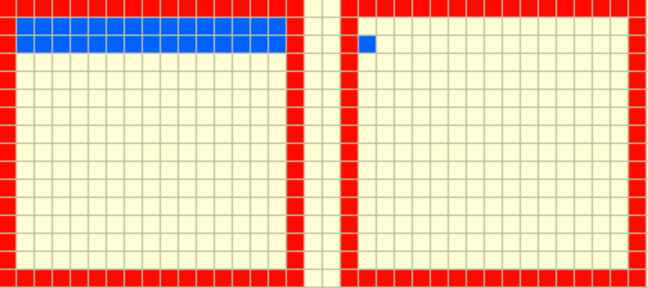
\includegraphics[scale=0.30]{figures/lu1a}\hspace{1em}
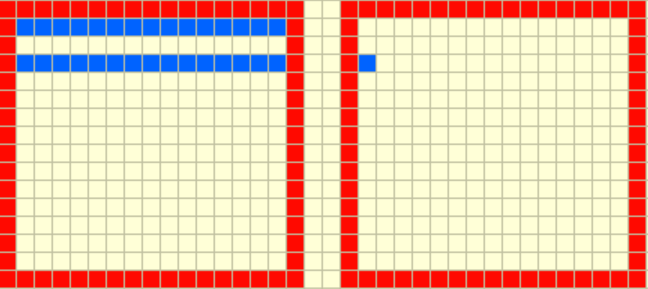
\includegraphics[scale=0.30]{figures/lu1b}
\hspace{1em}
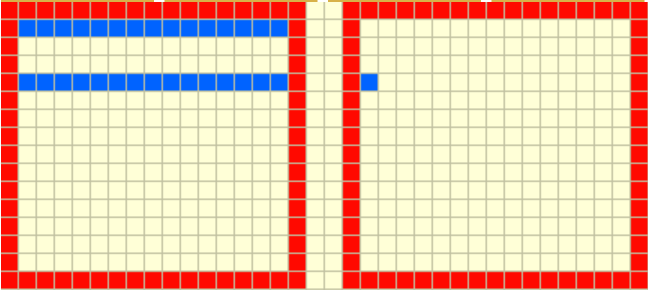
\includegraphics[scale=0.30]{figures/lu1c}
\hspace{1em}
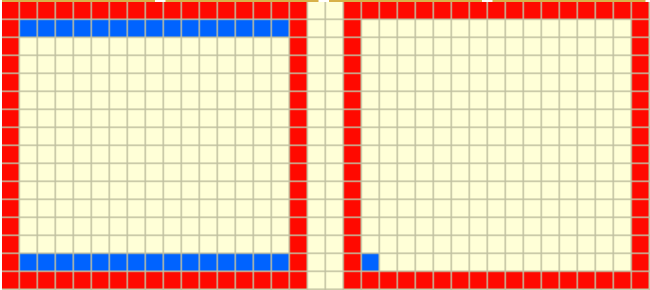
\includegraphics[scale=0.30]{figures/lu2} 


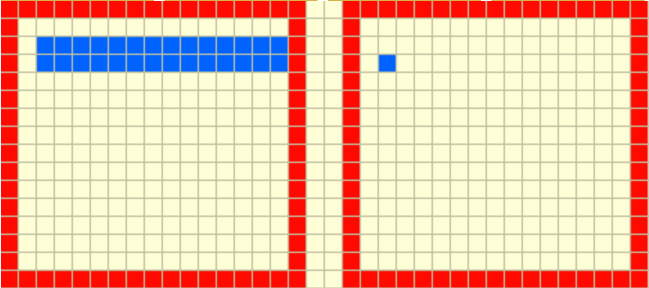
\includegraphics[scale=0.30]{figures/lu3}
\hspace{1em}
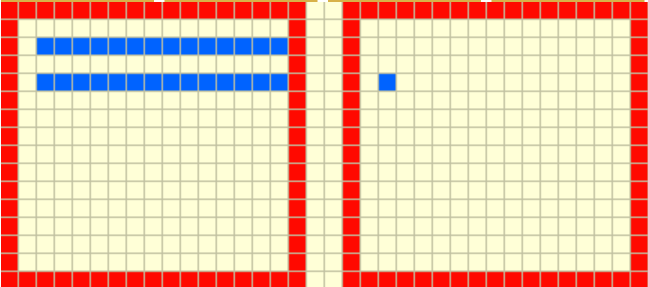
\includegraphics[scale=0.30]{figures/lu4}
\hspace{1em}
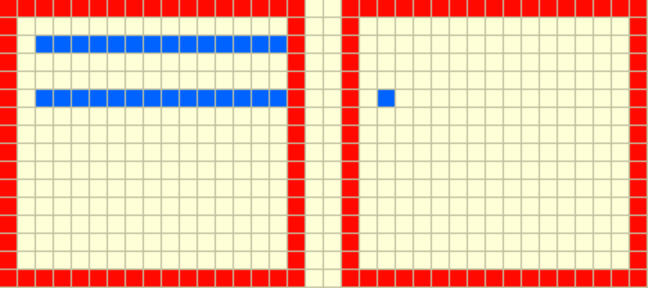
\includegraphics[scale=0.30]{figures/lu2b}
\hspace{1em}
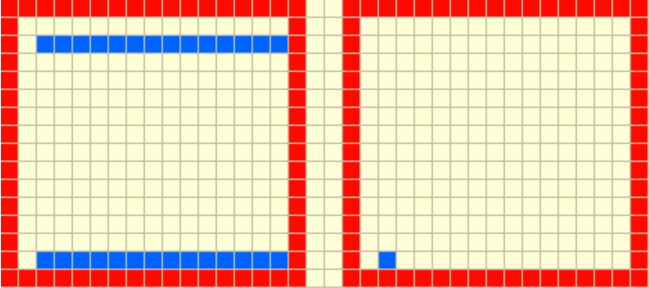
\includegraphics[scale=0.30]{figures/lu5}
$$\vdots$$
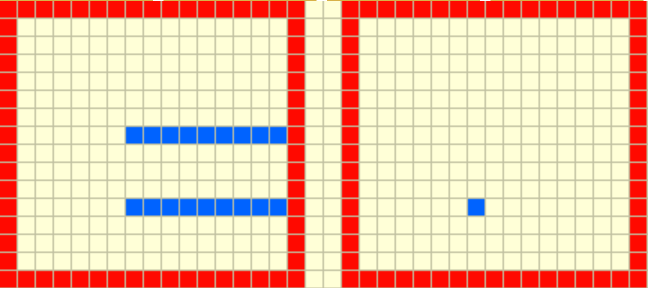
\includegraphics[scale=0.33]{figures/lu6}
$$\vdots$$
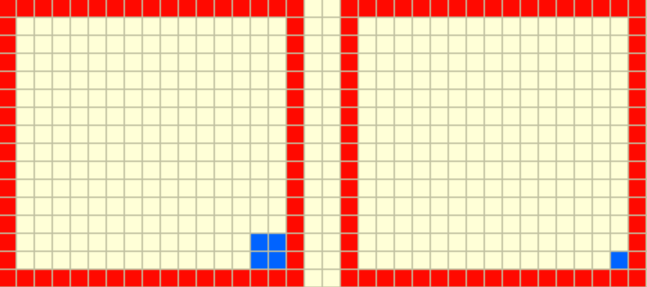
\includegraphics[scale=0.33]{figures/lu7}
\end{center}

\section{Existing Work}

\section{Approach}

We will start off with a simple implementation of LU factorization that is not optimized for any particular architecture which will serve as a starting point to measure performance improvements.


\subsection{Architecture}

Our initial optimizations target a multicore CPU architecture, such as the current Intel Haswell series i7 4970K processor. By utilizing OpenMP, our code will be accessible on a wide variety of platforms. This project may also utilize CUDA in order to implement parallel optimizations on the GPU. GPU parallelization is advantageous as it allows us to take advantage of a large number of cores + threads. Code optimizations will target the most recent nvidia GTX 970 GPU. 

\subsection{Optimizations}

TO-DO: cache, loop unrolling, openMP, vector operations, cuda

\section{Results}

\subsection{Sequential Optimizations}

\subsection{Parallel Optimizations}

\section{Conclusion}

>>>>>>> 36f274ab19dcce576b1e7f322dc88441edf3de78
\end{document}